\documentclass[8pt]{article}
\usepackage{amsmath, xfrac, enumitem, graphicx, ulem, float, bigints, bm, textcomp}
\usepackage[margin=0.7in]{geometry}
\graphicspath{ {images/} }
\title{Thermodynamics GATE}\author{Kulasekaran}
\linespread{0.8}
\begin{document}
\maketitle
\begin{center}
\subsection*{\uwave{1. Basic Concepts \& Zeroth Law of Thermodynamics}}
\end{center} 
%----------------------------------------------------------------------------------------%
\dashuline{\textbf{Macroscopic Approach}}\\
	\begin{itemize}
		\item Average molecular behaviour considered
		\item \textbf{Continumm} concept should be valid
			\begin{itemize}
				\item Matter is continuously distributed
				\item In case of gases, the \textbf{Mean Free Path} (average distance travelled by molecule between two successive collisions) should be less than system dimensions.
			\end{itemize}
	\end{itemize}\hrulefill\\
%----------------------------------------------------------------------------------------%
\\\dashuline{\textbf{Quasistatic process}} - Infinitely slow process. 
	\begin{itemize}
		\item All reversible processes are quasistatic, but not all quasistatic processes are reversible. 
		\item Frictionless quasistatic process is reversible
		\item Properties of a system are Exact differentials
	\end{itemize}
%----------------------------------------------------------------------------------------%
\hrulefill\\
\\\dashuline{\textbf{Intensive properties}}
	\begin{itemize}
		\item Independent of mass
		\item All specific properties like, specific volume, specific heat are Intensive properties. 
		\item Density is also an intensive property. 
		\item Intensive properties when divided will still be the same. 
	\end{itemize}\hrulefill\\
%----------------------------------------------------------------------------------------%
\\\dashuline{\textbf{Extensive properties}}
	\begin{itemize}
		\item Dependent on mass
		\item When divided will be half as before. 
	\end{itemize}\hrulefill\\\\
%----------------------------------------------------------------------------------------%
\dashuline{\textbf{Temperature Scales :-}}
	\begin{itemize}
		\item[] $\boxed{\dfrac{t_c-0}{100-0} = \dfrac{t_F-32}{212-32}}$
		\item Converting Degree Celcius to Fahrenheit $\implies\boxed{t_f = \dfrac{9}{5}t_c+32}$
		\item \textbf{Note:} $\boxed{\Delta t_F = 1.8\Delta t_C}$
	\end{itemize}\hrulefill\\\\
%----------------------------------------------------------------------------------------%
\dashuline{\textbf{Gibbs Phase rule :-}}
	\begin{itemize}
		\item $\boxed{P+F = C+2}$
			\begin{itemize}
				\item[$\rightarrow$] P = Number of Phases
				\item[$\rightarrow$] F = Degree of Freedom 
				\item[$\rightarrow$] C = Number of chemical components
			\end{itemize}
	\end{itemize}
%----------------------------------------------------------------------------------------%
\begin{itemize}
	\item[$\rightarrow$] Mixture of Refrigerants which behave as pure substance is called \textbf{Azeotrope}
	\item[$\rightarrow$] Mixture of Air and Liquid air is not a pure substance
	\item[$\rightarrow$] \textbf{Extensive properties are additive}, meaning extensive property's whole is the sum of parts of the extensive property.
\end{itemize}\hrulefill\\\\
%----------------------------------------------------------------------------------------%
\begin{center}
\subsection*{\uwave{2. Energy and Energy Interactions}}
\end{center}
$\rightarrow$ The molecular weight of air is approximamtely taken as 29. Air is approx 77\% of $N_2$ and 23\% $O_2$ by weight. So,
$$\boxed{0.77 * 28 + 0.23 * 32 = 28.92 \approx 29}$$\\
%----------------------------------------------------------------------------------------%
\\\dashuline{\textbf{Ideal Gas Equation}}\\
	\begin{itemize}
		\item $PV = mRT$ Where,
		\begin{itemize}
			\item P = Pressure
			\item V = Volume 
			\item m = Mass 
			\item R = Characteristic Gas Constant
			\item T = Temperature
		\end{itemize}
		\item Also $PV = n\bar{R}T$ Where,
		\begin{itemize}
			\item n = Number of Kilo moles
			\item $\bar{R}$ = Universal Gas Constant = 8.314 $\sfrac{KJ}{Kmol K}$			
		\end{itemize}
		\item Now, R for Air is calculated as: $R_{Air} = \dfrac{\bar{R}}{M_{Air}} = \dfrac{8.314}{29} = 0.287 \sfrac{KJ}{Kmol K}$
		\item $\boxed{mass(m) = number\;of\;moles(n) * Molecular\;mass(M)}$\\
	\end{itemize}\hrulefill\\\\
%----------------------------------------------------------------------------------------%
\\\dashuline{\textbf{Work}} - (+ve = Done by system, -ve = Done on system)
	\begin{itemize}
		\item The work done by a \textbf{reversible process or closed system process} is the area under the curve in a P-V diagram.
		\item The work done in a \textbf{reversible cycle or closed system cycle}    is the area enclosed by the curve in a P-V diagram.
	\end{itemize}
%-----------------------------------------------------------------------------------------%
\dashuline{\textbf{Work in various Quasi-static processes}}
	\begin{itemize}
		\item[1.] \textsc{Constant Volume - Isochoric - Isometric process} $\implies \boxed{W_{1-2} = 0}$
		\item[2.] \textsc{Constant Pressure - Isobaric - Isopiestic process} $\implies \boxed{W_{1-2}=\int _1^2 PdV = P(V_2-V_1)}$
			\begin{figure}[H]
				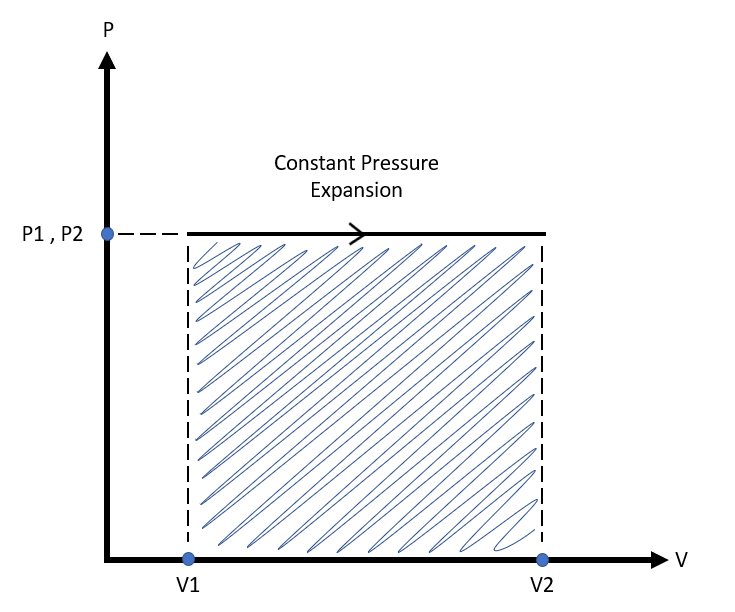
\includegraphics[scale=0.3]{constpress.png} 
				\centering
			\end{figure}\hrulefill\\
		\item[3.] \textsc{Constant Temperature - Isothermal - Hyperbolic process} $\implies \boxed{W_{1-2} = P_1V_1\ln \dfrac{V_2}{V_1} = P_1V_1\ln \dfrac{P_1}{P_2}}$
			\begin{figure}[H]
				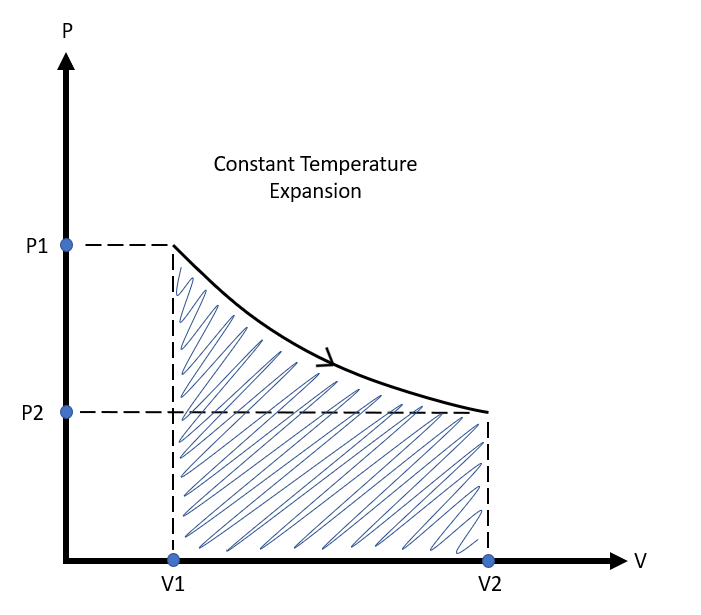
\includegraphics[scale=0.3]{consttemp.png} 
				\centering
			\end{figure}\hrulefill
		\item[4.] \textsc{Adiabatic process}  $\implies \boxed{W_{1-2} = \dfrac{P_1V_1-P_2V_2}{\gamma -1}}$ $\boxed{\dfrac{T_2}{T_1}=\left(\dfrac{P_2}{P_1}\right)^{\dfrac{\gamma -1}{\gamma}}=\left(\dfrac{V_1}{V_2}\right)^{\gamma -1}}$
			\begin{figure}[H]
				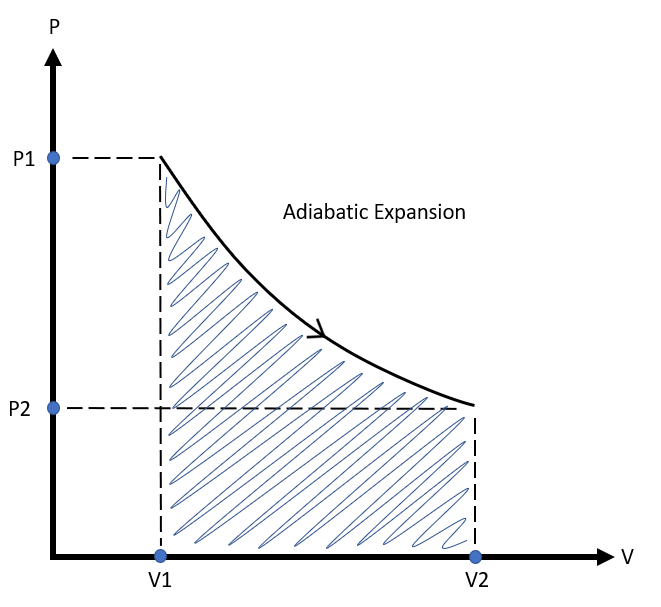
\includegraphics[scale=0.3]{adiabatic.png}
				\centering
			\end{figure}\hrulefill
		\item[5.] \textsc{Polytropic process}  $\implies \boxed{W_{1-2} = \dfrac{P_1V_1-P_2V_2}{n-1}}$ $\boxed{\dfrac{T_2}{T_1}=\left(\dfrac{P_2}{P_1}\right)^{\dfrac{n-1}{n}}=\left(\dfrac{V_1}{V_2}\right)^{n-1}}$
	\end{itemize}
	\hrulefill\\\\
%----------------------------------------------------------------------------------------%
\\\dashuline{\textbf{Heat}} - (+ve = Transferred to system, -ve = Rejected from system)
	\begin{itemize}
	\item The Heat transfer in a \textbf{reversible process} is the area under the curve in a T-S diagram
	\item The Heat transfer in a \textbf{ reversible cycle} is the area enclosed by the curve in a T-S diagram.
	\item The specific heats (Cp and Cv) of monoatomic gas is constant with temperature. They vary for Di and tri atomic gases
	\item We know $\boxed{\frac{C_P}{C_V}=\gamma}$. But $\gamma$ can also be calculate in another way: $\boxed{\gamma = 1+\frac{2}{n}}$
		\begin{itemize}
			\item n = Degree of freedom, T = Translational, R = Rotational
			\item n = 3 for mono atomic gases [3T]
			\item n = 5 for di atomic gases [3T+2R]
			\item n = 6 for tri atomic gases [3T+3R]
		\end{itemize}		 
	\item Heat capacity of the substance = Mass * Specific Heat
	\item \textsc{Latent heat}
		\begin{itemize}[wide]
			\item It is the Amount of Heat required to cause phase change in unit mass of any substance. It is of three types:
			\item \textbf{Latent heat of fusion ($L_f$)} $\rightarrow$ Not much affected by pressure
			\item \textbf{Latent heat of vapourization ($L_V$)} $\rightarrow$ Highly sensitive to pressure.
			\item \textbf{Latent heat of sublimation}
			\item \textbf{Very important thing to note is that, in these phase change scenarios, even when heat transfer is taking place, the temperature of the system remains constant}
			\item consider the scenario where a solid at temperature $T_1$ is to be converted into vapour at temperature $T_2$. The freezing temperature is $T_f$ and the boiling temperature is $T_V$. The total heat required for this conversion to occur is calculated as follows: Here ($T_1 < T_f$), ($T_2 > T_V$)
			\begin{itemize}
				\item Heat added to rasie temp from $T_1$ to $T_f$: $\boxed{Q_1 = mC_1(T_f-T_1)}$
				\item Heat added for phase change from Solid to Liquid: $\boxed{Q_2 = mL_f}$
				\item Heat added to raise temp from $T_f$ to $T_V$: $\boxed{Q_3 = mC_2(T_V-T_f)}$
				\item Heat added for phase change from Liquid to Vapour: $\boxed{Q_4 = mL_V}$
				\item Heat added to raise temp from $T_V$ to $T_2$: $\boxed{Q_5 = mC_3(T_2-T_V)}$
				\item Here, $C_1$,$C_2$,$C_3$ are specific heats of the substance in Solid, Liquid and Gaseous phases respectively.
				\item Total heat required for the aforementioned conversion is the sum of all the above heats from $Q_1$ to $Q_5$
			\end{itemize}
		\end{itemize}
	\item Increasing of order of slopes for the following processes in P-V diagram:$$\boxed{\textbf{Isothermal \textless \;Polytropic \textless \;Adiabatic}}$$
\end{itemize}
\hrulefill
%----------------------------------------------------------------------------------------%
\begin{center}
\subsection*{\uwave{3. First Law of Thermodynamics}}
\end{center}
\dashuline{\textbf{First Law :-}}\\
	\begin{itemize}
		\item $dE = dU + dK.E. + dP.E.$
		\item $\delta W = \delta W_{PdV} + \delta W_{shaft} + \delta W_{elec} $
		\item $\delta Q = dE + \delta W$ for process
			\begin{itemize}
				\item[$\implies$] $\boxed{\delta Q = dU + \delta W}$ for stationary process
			\end{itemize}
		\item $\delta Q = \delta W \impliedby$ [for cycle ($dU = 0$)]
		\item $U(Internal\;energy),H(Enthalpy) = f(T)$ only for an ideal gas.	
	\end{itemize}\hrulefill\\\\
%----------------------------------------------------------------------------------------%
\dashuline{\textbf{Heat Transfer in Various processes :-}}\\\\
\textsc{Constant Volume}
	\begin{itemize}
		\item from first law, $\delta Q = dU + \delta W \implies dU + PdV \implies dU + 0$
		\item $\implies \delta Q = dU = mC_V\Delta T$
	\end{itemize}\hrulefill\\\\
%----------------------------------------------------------------------------------------%
\textsc{Constant pressure}
	\begin{itemize}
		\item \textbf{Enthalpy}(H) = U + PV
		\item In constant pressure proces, from First law, $\delta Q = dU + \delta W \implies dU + PdV \implies dU + dPV \implies d(U+PV) = dH$
		\item $\implies \delta Q = dH = mC_p\Delta T \impliedby$ applicable in cases of constant pressure process or Ideal gas involving any process
	\end{itemize}\hrulefill\\\\
%----------------------------------------------------------------------------------------%
\textsc{Constant Temperature}
	\begin{itemize}
		\item In case of constant temperature, dU = 0. So, $\delta Q = \delta W$
		\item \textbf{NOTE: } The above is not possible due the limitations of second law.
	\end{itemize}\hrulefill\\\\
%----------------------------------------------------------------------------------------%
\textsc{Adiabatic Heat transfer}
	\begin{itemize}
		\item Since, its adiabatic, $\delta Q = 0 \implies W = -dU = U_1 - U_2$
	\end{itemize}\hrulefill\\\\
%----------------------------------------------------------------------------------------%
\textsc{Polytropic Heat transfer}
	\begin{itemize}
		\item $Q_{poly} = W_{poly}*\left(\dfrac{\gamma -n}{\gamma -1}\right) \implies \boxed{\dfrac{P_1V_1-P_2V_2}{n-1}*\left(\dfrac{\gamma -n}{\gamma -1}\right)}$
		\item Specific heat for polytropic process, $\boxed{C_{poly} = -C_V*\left(\dfrac{\gamma -n}{n-1}\right)}$
		\item the above is derived using the first law and Meyer's equation: $C_P-C_V=R$. This relation is derived from the definition of enthalpy as H = U + PV $\implies mC_PdT = mC_VdT + mRdT$
			\begin{itemize}
				\item[$\implies$] $C_V = \dfrac{R}{\gamma -1}$ and $C_P = \dfrac{\gamma R}{\gamma -1}$
			\end{itemize}
		\item Polytropic specific heat being negative implies that even though heat is added to the gas, its temperature decreases because the work done by the gas exceeds the heat supplied to the gas and the additional work is done at the expense of the internal energy
		\item Generally $1 < n < \gamma$
	\end{itemize}\hrulefill\\\\
%----------------------------------------------------------------------------------------%
\dashuline{\textbf{Free Expansion of gases}}\\
	\begin{itemize}[wide]
		\item The free expansion process is \textbf{highly irreversible} 
		\item When partition is removed the internal energy of the fluid gets used as Kinetic energy
		\item When the particles hit the walls of the container and reaches the equilibrium, the Kinetic energy gets converted back into Internal energy
		\item Even though the Initial and final internal energy is same, meaning Initial and final temperature is same, the process is not isothermal, because when the fluid is expanding with Kinetic energy, the temperature varies.
		\item \textbf{Note:} Instead of partition, if there is movable frictionless piston, it is \textbf{not the case of free expansion}, as the fluid is doing work on the piston. here also the final and initial temperature will be same.
	\end{itemize}
\hrulefill
%----------------------------------------------------------------------------------------%
\begin{center}
\subsection*{\uwave{4. Open System Analysis by First Law}}
\end{center}
$$\boxed{\textbf{SFEE} \implies U_1 + P_1V_1 + \dfrac{{C_1}^2}{2} + gZ_1 + Q = U_2 + P_2V_2 + \dfrac{{C_2}^2}{2} + gZ_2 + W_{CV}}$$
\\\dashuline{\textbf{Steady Flow systems}}\\
	\begin{itemize}
		\item Fluid properties can change from point to point within the control volume, but they don't change with respect to time
		\item The volume, mass and total energy of the control volume remain constant. As a result, the displacement work is zero as V is constant. 
		\item Mass balance equation: Mass incoming = Mass outgoing. That is $\boxed{\sum_{inlet} \dot{m}_i = \sum_{outlet}\dot{m}_e}$
		\item \textbf{NOTE:} In case of Air as the fluid, the continuity equation is $\boxed{\rho_1A_1V_1 = \rho_2A_2V_2}$ 
		\item \textbf{NOTE:} But in case of Liquids(Incompressible fluids), the continuity equation is $\boxed{A_1V_1 = A_2V_2}$
	\end{itemize}
\hrulefill\\
%----------------------------------------------------------------------------------------%
\\\dashuline{\textbf{Nozzle \& Diffusers}}
	\begin{itemize}
		\item Assumptions:
		\begin{itemize}
			\item $\Delta PE = 0$ i.e $Z_1 - Z_2 = 0$
			\item Adiabatic process (Nozzle is insulated) $\implies$ Q=0;
			\item $W_{CV} = 0$
		\end{itemize}
		\item So, SFEE = $\boxed{h1 + \dfrac{{C_1}^2}{2} = h2 + \dfrac{{C_2}^2}{2}}$
		\item \textbf{NOTE:} Generally the enthalpies in the sum will be given in KJ/kg which has to be converted to J/Kg to get the velocities in m/s.
	\end{itemize}
\hrulefill\\
%----------------------------------------------------------------------------------------%
\\\dashuline{\textbf{Turbine and Compressors}}
	\begin{itemize}
		\item Assumptions:
			\begin{itemize}
				\item Insulated $\implies$ Q = 0;
				\item Flow velocities are negligible $\implies$ C1 = C2 = 0;
				\item $Z_2 - Z_1$ also negligible $\Delta PE = 0$
			\end{itemize}
		\item So, SFEE = $\boxed{h_1 = h_2 + W_{CV}}$
		\item For Turbines, $W_{CV}$ is positive. For compressor, its negative. 
	\end{itemize}	
\hrulefill\\
%----------------------------------------------------------------------------------------%
\\\dashuline{\textbf{Throttling}} (Pressure drop)
	\begin{itemize}
		\item Assumptions
			\begin{itemize}
				\item Adiabatic $\implies$ Q = 0;
				\item No workdone $\implies W_{CV} = 0$
				\item K.E. = 0 \& P.E. = 0 
			\end{itemize}				
			\item So, SFEE $\implies \boxed{h_1 = h_2}$ - Since the enthalpy at inlet and outlet are same, the throttling valves are referred to as \textbf{Isenthalpic valves}
			\item Dryness friction(x)
				\begin{itemize}
					\item SFEE $\implies \boxed{h_1 = h_f + x(h_g - h_f)}$
				\end{itemize}
	\end{itemize}
\hrulefill	\\
%----------------------------------------------------------------------------------------%
\\\dashuline{\textbf{Heat Exchangers}}
	\begin{itemize}
		\item Assumptions
			\begin{itemize}
				\item Heat exchange is within the CV. So, no heat interactions with the surroundings. $\implies$ Q = 0;
				\item No workdone $\implies W_{CV} = 0$
				\item K.E. = 0 \& P.E. = 0 
			\end{itemize}
		\item So, SFEE for (non-contact type - hot and cold fluid do not mix) $$\implies \boxed{\dot{m}_ch_1 + \dot{m}_hh_2 = \dot{m}_ch_3 + \dot{m}_hh_4}$$
		\item So, SFEE for (contact type - hot and cold fluid mix) $\implies \boxed{\dot{m}_1h_1 + \dot{m}_2h_2 = \dot{m}_3h_3}$
	\end{itemize}
	\hrulefill\\
%----------------------------------------------------------------------------------------%
\\\dashuline{\textbf{Comparison of SFEE with Euler and Bernoulli's equation}}
\begin{align*}
		\textbf{SFEE} &\implies U_1 + P_1V_1 + \dfrac{{C_1}^2}{2} + gZ_1 + Q = U_2 + P_2V_2 + \dfrac{{C_2}^2}{2} + gZ_2 + W_{CV}\\
		&\implies H_1 + \dfrac{{C_1}^2}{2} + gZ_1 + Q = H_2 + \dfrac{{C_2}^2}{2} + gZ_2 + W_{CV}\\
		&\implies h_1 + \dfrac{{C_1}^2}{2} + gZ_1 + \delta q = h_2 + \dfrac{{C_2}^2}{2} + gZ_2 + \delta w_{CV}
\end{align*}
\hspace{2cm} where $h_1, h_2$ $\delta q$ and $\delta w_{CV}$ are specific quantities, i.e., they are divided by mass(m)
\begin{align*}
	&\implies \delta q = -h_1 + -\dfrac{{C_1}^2}{2} + -gZ_1 + h_2 + \dfrac{{C_2}^2}{2} + gZ_2 + \delta w_{CV}\\
	&\implies \delta q = (h_2-h_1) + \dfrac{{C_2}^2 - {C_1}^2}{2} + g(Z_2-Z_1) + \delta w_{CV}
\end{align*}
\begin{itemize}
	\item $(h_2-h_1)=dH$
	\item $(z_2-z_1)=dz$
	\item $\dfrac{{C_2}^2 - {C_1}^2}{2}=CdC$
	\item \textbf{Assumptions:}
		\begin{itemize}
			\item Insulated. $\implies \delta q = 0$
			\item No Work done $\implies \delta w_{CV} = 0$
			\item Temperature remains constant $\implies du = 0$
			\item Fluid is incompressible $\implies dv = 0$  
		\end{itemize}
\end{itemize}
\begin{align*}
	\implies 0 &= dh + CdC + gdZ + 0\\
	&=du + Pdv + vdP + CdC + gdZ\\
	&=0 + 0 + \boxed{vdP + CdC + gdZ} --- Euler's\;form\;of\;SFEE
\end{align*}
Integration of the above between two section will give the Bernoulli's form of SFEE:
$$\boxed{\dfrac{P_1}{\rho} + \dfrac{{C_1}^2}{2} + gZ_1 = \dfrac{P_2}{\rho} + \dfrac{{C_2}^2}{2} + gZ_2}$$
\hrulefill\\
%----------------------------------------------------------------------------------------%
\\\dashuline{\textbf{Unsteady flow}}
	\begin{itemize}
		\item The rate at which mass of fluid within the control volume is accumulated is equal to the net rate of mass flow across the control surface $\implies \dfrac{dm_{cv}}{dt} = \dot{m}_i - \dot{m}_e$
		\item Similarly $\implies \dfrac{dE_{cv}}{dt} = \dot{E}_i - \dot{E}_e$
		\item So, $\boxed{\dfrac{dE_{cv}}{dt} = \left\{\dot{m}_i  \left(h_i + \dfrac{{C_i}^2}{2} + gZ_i \right) + \dot{Q} \right\} - \left\{\dot{m}_e\left(h_e + \dfrac{{C_e}^2}{2} + gZ_e\right) + \dot{W_{CV}} \right\}  }$
		\item The above is called the \textbf{First law of thermodynamics for an open system with Unsteady flow}
		\item If the above system is stationary, then $\implies\boxed{\dfrac{dE_{cv}}{dt} = \dfrac{dU_{cv}}{dt} = \dot{m}_ih_i + \dot{Q} - \dot{m}_eh_e - \dot{W}_{CV}}$
	\end{itemize}
	\hrulefill\\
%----------------------------------------------------------------------------------------%
\\\dashuline{\textbf{Charging of tank}}
	\begin{itemize}
		\item a supply line carrying a fluid in connected to a \textbf{rigid, isolated and evacuated} tank.
		\item No changes in K.E. and P.E. 
		\item No Work done
		\item No heat interactions (as Insulated)
		\item Since there is no exit, the rate of change of mass inside the tank is given by:
		$$\implies \dfrac{dm_{CV}}{dt} = \dot{m}_i \;\;\; \implies \dfrac{dU_{CV}}{dt} = \dot{m}_ih_i$$
		\item Assuming $h_i$ as constant and integrating will give us:
		$$\implies (U_f - U_i)_{CV} = h_i(m_f)_{CV}\;\;\;(U_i = 0,\;U_f = u_f * m_f)$$
		$$So,\;\boxed{u_f = h_i}\;\;\;(u_f = c_v*T_f,\;\;h_i=c_p*T_f)$$
		$$\implies \boxed{T_f = \gamma*T_i}$$
	\end{itemize}
\hrulefill
%----------------------------------------------------------------------------------------%
\begin{center}
\subsection*{\uwave{5. Second Law of Thermodynamics}}
\end{center}
\dashuline{\textbf{Thermal Energy Reservoir (TER)}}\\
		\begin{itemize}[labelindent=1cm, leftmargin=1cm, wide]
			\item A hypothetical body with large heat capacity (mass * SpecificHeat) that can supply or absorb large amounts of heat with not much change in its temperature. Example: The air in a room with a TV as a heating source can be considered as a TER
		\end{itemize}
		\hrulefill\\
%----------------------------------------------------------------------------------------%
\\\dashuline{\textbf{Heat engines}}
		\begin{itemize}[wide]
			\item Rotating a paddle shaft in water will increase the internal energy of the water, which will later leave the water as heat. So, work gets converted into heat naturally. 
			\item But the reverse requires usage of special devices called \textbf{Heat engines} which takes in heat as input and produce work. 
			\item There are different types of heat engines, but they have common charateristics like, they absorb heat from a source,\textbf{ convert a part of it as work and reject remaining} to the sink
			\item \textbf{Example:} Steam powerplant is a heat engine. It has five major components: Furnace, Boiler, Turbine, Condenser, Pump. The boiler takes in heat from the furnace, heats up the water to convert it to steam, the steam runs the turbine and generate work, then gets condensed back to water by the condenser and the pump pushes the water back into the boiler.  
		\end{itemize}
		\hrulefill\\
%----------------------------------------------------------------------------------------%
\\\dashuline{\textbf{Thermal Efficiency ($\eta$)}}
		\begin{itemize}[wide]
			\item The ratio of fraction of heat that gets converted as work, to the total heat input to the boiler is called as the Thermal efficiency of the Heat engine. 
			\item $\boxed{\eta=\dfrac{W_{net}}{Q_{supplied}}}$	
			\item $\delta Q_{net} =$ Amount of heat supplied to boiler$(Q_1)$ - Amount of heat rejeted from condenser$(Q_2)$
			\item $\delta W_{net} =$ Amount of Work produced by Turbine$(W_1)$ - Amount of work required by pump to get water back to boiler pressure$(W_2)$	
			\item In a cyclic process, $\Delta U = 0$. So, according to first law, $\delta Q = \delta W \implies \delta Q_{net} = \delta W_{net}$
			\item So, $\eta = \dfrac{W_{net}}{Q_1} \implies \dfrac{Q_{net}}{Q_1} \implies \dfrac{Q_1 - Q_2}{Q_1} \implies \boxed{1 - \dfrac{Q_2}{Q_1}}$
			\item Thermal efficiency of 100 percent is impossible in reality.  For $\eta = 100\%\; Q_2$ has to be Zero. I.e., There must be zero heat loss and all of heat input should be converted to work.   
		\end{itemize}
		\hrulefill\\
%----------------------------------------------------------------------------------------%	
\\\dashuline{\textbf{Kelvin-Planck Statement}}
			\begin{itemize}[wide]
				\item \textit{" It is impossible for a system to operate in a thermodynamic cycle and deliver a net amount of energy by work to its surroundings while receiving energy by heat transfer from a single reservoir "}
				\item In simple terms, Thermal efficiency can never be 100\%.
			\end{itemize}
		\hrulefill\\
%----------------------------------------------------------------------------------------%		
\\\dashuline{\textbf{Perpetual Motion Machine}}
			\begin{itemize}
				\item \textbf{PMM - I}: A machine that violates first law of thermodynamics - Producing work without Heat. $\implies \delta Q \neq \delta W$
				\item \textbf{PMM - II}: A machine that violates second law of thermodynamics (Kelvin-planck) - 100\% Thermal efficiency
				\item \textbf{PMM - III}: A machine that works continuously without any heat or work interaction with the surrounding. This is possible only in the complete absence of all forms of irreversibitlies. 
			\end{itemize}
			\hrulefill\\
%----------------------------------------------------------------------------------------%		
\\\dashuline{\textbf{Refrigerators and Heat pumps}}
			\begin{itemize}[wide]
				\item Heat tranfer from high temp to low temp can occur naturally. But for the reverse to occur, special devices like \textbf{Refrigerator or Heat pump} is required.
				\begin{itemize}
%----------------------------------------------------------------------------------------%
					\item \textsc{Refrigerator}
						\begin{itemize}[wide]
							\item Like Heat engine which uses water as the working fluid, refrigerators use refrigerants as working fluid. \textbf{Vapor compression refrigeration} is one of the most commonly used process. 
							\item It has four main components: Compressor, condensor, expansion valve (capillary tube) and evaporator. 
							\item The refrigerant enters the compressor (the compressor requires external work) and gets its pressure increased. Then it enters the condensor where its temperature decreases by rejected heat to the surrounding. Then it goes through an expansion valve, where due to throttling its pressure and temperature drop significantly. Then the refrigerant enters the evaporator where it absorbs heat from the surrounding and re-enters the compressor.
							\item $Q_L$ - Amount of heat removed from refrigerated space which is at temperature $T_L$
							\item $Q_H$ - Amount of heat rejected from condensor to surrounding which is at a temperature of $T_H$
							\item $W_{net}$ - Work input to the compressor. 
							\item $Q_H - Q_L = W_{net} \implies \boxed{Q_H = W_{net} + Q_L}$
							\item $\boxed{COP_R = \dfrac{Desired\;effect}{Work\;input} \implies \dfrac{Q_L}{W_{net}} \implies \dfrac{Q_L}{Q_H-Q_L}}$\\
						\end{itemize}
					
%----------------------------------------------------------------------------------------%
					\item \textsc{Heat Pumps}
						\begin{itemize}[wide]
							\item Heat pump is another device that transfers heat from low temp to high temp. But the operation objective of heat pump is different from that of refrigerator as it is used to make the place warmer than surroundings whereas refrigerator makes a space colder than surroundings. 
							\item $\boxed{COP_H = \dfrac{Q_H}{W_{net}} \implies \dfrac{Q_H}{Q_H-Q_L}}$ \textbf{NOTE:} $\boxed{COP_H=COP_R+1}$
						\end{itemize}
					\end{itemize}
				\end{itemize}		 
			\hrulefill\\\pagebreak
%----------------------------------------------------------------------------------------%
\\\dashuline{\textbf{Clausius Statement :-}}
			\begin{itemize}
				\item Heat pumps and refrigerators are based on clausius statement of second law of thermodynamics
				\item \textit{" It is immpossible to construct a device that operates in a cycle and produces no effect other than the transfer of heat from a lower-temperature body to a higher temperature body "}
				\item In simple terms, Transfer of heat from low temperature to high temperature without the aid of an external agency is impossible. 
				\item According to Clausius statement, \textbf{NOTE:} $COP_H$ and $COP_R$ can never be $\infty$	
			\end{itemize}				
	\hrulefill\\
%----------------------------------------------------------------------------------------%
\\\dashuline{\textbf{Reversible process :-}}
		\begin{itemize}
			\item They do not occur in nature due to second law of thermodynamics. 
			\item They need to be carried out infinitely slowly (Quasi-static)
			\item Since they don't occur in nature, devices imagined to be performing reverible processes have the best efficiency compared to the ones performing 	Irreversible processes. It applies to both work-producing as well as work-consuming devices.
			\item concept of reversibility leads to \textbf{Second Law efficiency} for actual processes which tells by what percent the process is like a reversible process.
			\item \textbf{Internally Reversible}: If in a process, the system can be brought to its original state, then its called Internally Reversible
			\item \textbf{Externally Reversible}: If in a process, the surrounding can be brought to its original state, then its called Externally reversible 
		\end{itemize}
\hrulefill\\
%----------------------------------------------------------------------------------------%
\\\dashuline{\textbf{Irreversible process :-}}
		\begin{itemize}
			\item Factors like friction, free expansions, inelastic deformation, etc., create irreversibilites in processes.
			\item \textbf{Friction} - a brick is in contact with the floor. Moving the brick requires force which should be greater than the friction force between the brick and the floor. When applied force is higher than the firctional force, the brick will start moving. But since there is friction, heat will be generated due to motion, and this in turn will rasie the temperature of the body. Now if we try to bring back the body to its original position, still some more amount of heat will be generated since frictional force is always opposite to the direction of motion. Those heats that were generated will get dissipated into the surrounding (considereing the brick to be the system). 
		\end{itemize}
		\hrulefill\\	%----------------------------------------------------------------------------------------%
\\\dashuline{\textbf{Carnot Cycle :-}}
		\begin{itemize}
			\item Carnot cycle is composed of an \textbf{adiabatic piston cyclinder with gas inside} 
			\item Processes:
				\begin{itemize}
					\item (1-2) Reversible isothermal heat addition: $\boxed{Q_H = (U_2-U_1)+W_{1-2}}$
					\item (2-3) Reversible adiabatic expansion: $\boxed{0 = (U_3-U_2)+W_{2-3}}$
					\item (3-4) Reversible isothermal heat rejection: $\boxed{-Q_L=(U_4-U_3)-W_{3-4}}$
					\item (4-1) Reversible adiabatic compression: $\boxed{0=(U_1-U_4)-W_{4-1}}$				
					\begin{figure}[H]
						\includegraphics[scale=0.3]{carnot_combined.png}
						\centering
					\end{figure}
				\end{itemize}
			\item Carnot cycle cannot be used in actual devices because it becomes impractical to have a reversible isothermal heat transfer process, cause the heat transfer has to occur between infinitesimally small temperature difference and infinitely slowly. 
			\item A practical and slightly modified version of the carnot cycle is the \textbf{Rankine cycle} used in Steam plants. 
		\end{itemize}
		\hrulefill\\
%----------------------------------------------------------------------------------------%
\\\dashuline{\textbf{Reversed Carnot Cycle :-}}
		\begin{itemize}
			\item If all the process in carnot cycle is reversed, we obtain what is called a reversed carnot cycle or \textbf{Carnot Refrigeration cycle} which can be used for Heat pumps and refrigerators
		\end{itemize}
		\hrulefill\\	%----------------------------------------------------------------------------------------%
\\\dashuline{\textbf{Carnot Principles :-}}
		\begin{itemize}
			\item \textbf{Principle I:} $\boxed{\eta _{Rev} > \eta _{Irr}}$ for operation between the same temperature range
			\item \textbf{Principle II:} Efficiencies of all reversible engines working between the same temperature range are equal
		\end{itemize}
		\hrulefill\\
%----------------------------------------------------------------------------------------%
\\\dashuline{\textbf{Thermodynamic Temperature scale :-}}
		\begin{itemize}
			\item A temperature scale independent of the properties of the substances that are used to measure the temperature. 
			\item From carnot's principle II, the efficiency is dependent on the operating temperature range only, i.e,. $\boxed{\eta _{REV} = f(T_H, T_L)}$
			\item We know $\eta = 1 - \dfrac{Q_L}{Q_H}$. This can be written as: $\eta = 1-\dfrac{\Phi (T_L)}{\Phi (T_H)}$. Kelvin suggested, $\Phi(T)=T$. 
			\item So, $\boxed{\eta = 1-\dfrac{T_L}{T_H}}$
			\item And since $\eta$ cannot be 1, the lowest possible temperature for $T_L$ is Zero. Hence the Kelvin scale is called as absolute scale. 
			\item \textbf{NOTE:} We now know $\boxed{\dfrac{Q_L}{Q_H}=\dfrac{T_L}{T_H}}$ So, inorder to reach absolute zero, we would need heat rejected to the sink to be zero which would violate the Kelvin-planck statement of second law.  
		\end{itemize}
	\hrulefill\\
%----------------------------------------------------------------------------------------%
\\\dashuline{\textbf{Maximum performance measures for cycles operating between two reservoirs :-}}
		\begin{itemize}
			\item \textsc{Effect of temperature on performance of \textbf{reversible} devices}
				\begin{itemize}
					\item \textbf{Heat engine} $\implies\boxed{\eta = 1-\dfrac{T_L}{T_H}} \implies \eta \uparrow$ for $T_L\downarrow$ (or) $T_H\uparrow$. 
					\item Decreasing the $T_L\downarrow$ is more effective than increasing the $T_H\uparrow$
					\item \textbf{Refrigerator} $\implies\boxed{COP_R=\dfrac{T_L}{T_H-T_L} = \dfrac{1}{\left(\dfrac{T_H}{T_L}-1\right)}} \implies COP_R \uparrow$ for $T_L\uparrow$ (or) $T_H\downarrow$
					\item \textbf{Heat Pump} $\implies\boxed{COP_H=\dfrac{T_H}{T_H-T_L} = \dfrac{1}{\left(1-\dfrac{T_L}{T_H}\right)}} \implies COP_H \uparrow$ for $T_L\uparrow$ (or) $T_H\downarrow$
					\item For Refrigerator and Heat pump, increasing the $T_L\uparrow$ is more effective rather than decreasing the $T_H\downarrow$	
				\end{itemize}
	\end{itemize}\hrulefill
%----------------------------------------------------------------------------------------%
\begin{center}
\subsection*{\uwave{6. Entropy}}
\end{center}
\dashuline{\textbf{Clausius Inequality :-}}\\
	\begin{itemize}
		\item Entropy is a measure of Irreversibility
		\item Clausius inequality = $\boxed{\oint \dfrac{\delta Q}{T}\le 0} \implies \boxed{\oint \dfrac{\delta Q}{T} = 0}$ \hspace{0.5cm} $\boxed{\oint \dfrac{\delta Q}{T} < 0}$ \hspace{0.5cm} $\boxed{\oint \dfrac{\delta Q}{T} > 0}$ 
			\begin{itemize}
				\item[] \hspace{5.5cm}Reversible\hspace{1cm}Irreversible\hspace{1cm}Impossible
			\end{itemize}
	\end{itemize}
	\hrulefill\\
%----------------------------------------------------------------------------------------%
\\\dashuline{\textbf{The property of Entropy :-}}
	\begin{itemize}
		\item Just like how energy was defined using first law, entropy can be defined using clausius inequality. 
		\begin{figure}[H]
			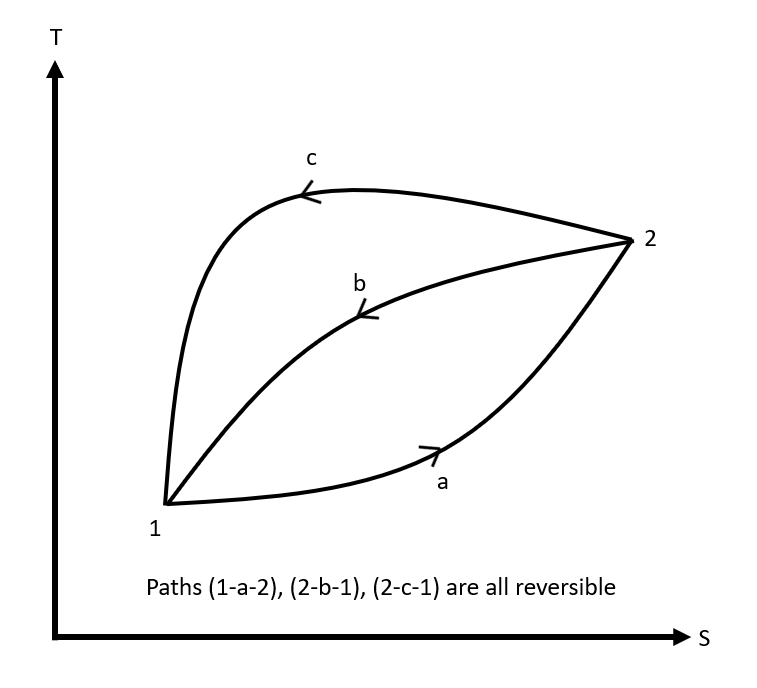
\includegraphics[scale=0.3]{entropy.png}
			\centering
		\end{figure}
		\item So, $\bigintss \limits_{2b1}\dfrac{\delta Q}{T} = \bigintss \limits_{2c1}\dfrac{\delta Q}{T}$, which means $\left(\dfrac{\delta Q}{T}\right)_{rev}$ must represent a property, which we are defining as Entropy(S).
		\item $S_2-S_1=\Delta S=\bigintss\limits_1^2dS=\bigintss\limits_1^2\left(\dfrac{\delta Q}{T}\right)_{rev}$ (Only for Reversible processes)
		\item \textbf{NOTE: }We have defined change in entropy instead of entropoy just like how we defined change in energy instead of energy itself. 
		\item Entropy is \textbf{Extensive} property
		\end{itemize}
		\hrulefill\\
%----------------------------------------------------------------------------------------%
\\\dashuline{\textbf{Entropy Increase} :-}
	\begin{itemize}
		\item If in the above diagram, \textbf{had the path C been irreversible}, Then 
		\item $\bigointss\limits_{1a2b1}\dfrac{\delta Q}{T} = 0$ but, $\bigointss\limits_{1a2c1}\dfrac{\delta Q}{T} < 0$ as it is irreversible.
		\item $\bigintss\limits_{2b1}\dfrac{\delta Q}{T} > \bigintss\limits_{2c1}\dfrac{\delta Q}{T} \implies \bigintss\limits_1^2dS > \bigintss\limits_{2c1}\dfrac{\delta Q}{T}$
		\item Which can be generalized as: $\boxed{dS \ge \dfrac{\delta Q}{T}}$
		\item The entropy change is equal to heat transfer in case of reversible process and in case of irreversible process, it is greater than it, which implies that \textbf{some entropy is generated during an irreversible process}.
		\item So, $\boxed{\Delta S_{sys} = S_2-S_1 = \int\limits_1^2\dfrac{\delta Q}{T}+\bm{S_{gen}}}$ $S_{gen}$ is always $\ge$ 0. $S_{gen}$ is a measure of magnitude of irreversibilities 
		\item \textbf{NOTE: }Unlike entropy, which doesn't depend on the path, the $\bm{S_{gen}}$ is a path function so it depends on the path. 
		\item In case of an \textbf{Isolated system}, $\boxed{\Delta S_{sys} = S_{gen}}$ and since $S_{gen}$ is always positive, the entropy of the universe always increases or incase of the never naturally occuring reversible process, it could remain constant, \textbf{but it could never decrease}. This is called \textbf{Increasing entropy principle}
		\item \textbf{NOTE: }The above principle does not mean that change in entropy cannot be negative. It only means that entropy generation can never be negative. 
		\item \textbf{NOTE: }Since entropy is an extensive property, total entropy = sum of parts of entropies of the system. $$\implies \boxed{S_{gen} = \Delta S_{univ} = \Delta S_{isolated}= \Delta S_{total} = \left(\Delta S_{Sys} + \Delta S_{Surr}\right) \ge 0}$$
	\end{itemize}
	\hrulefill\\
%----------------------------------------------------------------------------------------%
\\\dashuline{\textbf{T-S diagram :-}}	
	\begin{itemize}
		\item We know $\boxed{dS=\left(\dfrac{\delta Q}{T}\right)_{rev}}$. So, $\boxed{\delta Q_{rev} = TdS} \impliedby$ \textbf{Very important!!}
		\item $\implies \boxed{Q_{rev} = \int\limits_1^2Tds}$. Therefore, we can say area under the curve on a T-S diagram represent the heat transfer during a reversible process. 
		\item 	In case of an adiabatic process, there is no heat transfer, so
			\begin{itemize}
				\item[i.]Reversible adiabatic $\implies$ dS = 0. $\impliedby$ Isentropic process
				\item[ii.]Irreversible adiabatic $\implies$ dS = $S_{gen}$
			\end{itemize}
		\item From first law, $\delta Q = dU + \delta W$ and now we know, for a reversible process, $\delta Q = TdS$ \& $\delta W = PdV$. So, $\bm{TdS = dU + PdV}$
		\item And for a reverible cyclic process, $\bm{TdS = PdV}$ as $dU$ is zero in a cyclic process. So, for a cyclic process, \textbf{net heat interaction = net work interaction}
	\end{itemize}\hrulefill\\
%----------------------------------------------------------------------------------------%
\\\dashuline{\textbf{T-dS Relations :-}}
	\begin{itemize}
		\item[1.] $\boxed{TdS = dU + PdV}$
		\item[2.] $\boxed{TdS = dH - VdP} \impliedby \left(H = U + PV \implies dH = dU + PdV + VdP \implies dH = TdS + VdP\right)$
		\item \textbf{NOTE:} Even though the above relation is developed based on reversibility, since entropy is a point function, the above relations hold good for irreversible processes as well. 
		\item They can be applied to both closed / open systems as well. 
	\end{itemize}\hrulefill\\
%----------------------------------------------------------------------------------------%
\\\dashuline{\textbf{Slopes of Isobaric and Isochoric processes in T-S diagram :-}}
	\begin{itemize}
		\item For an Isochoric / Constant volume process, V = Constant. So, $TdS = dU + PdV \implies TdS = dU + 0 \implies TdS = mC_VdT$
			\begin{itemize}
				\item[] $\implies \boxed{\dfrac{dT}{dS}=\dfrac{T}{C_V}} \impliedby \left(\dfrac{dT}{dS} = Slope\;of\;a\;curve\;in\;TS\;diagram. \right)$
			\end{itemize}
		\item For an Isobaric / Constant pressure process, P = Constant, So, $dH = TdS + VdP \implies dH = TdS + 0 \implies mC_pdT = TdS$
			\begin{itemize}
				\item[] $\implies \boxed{\dfrac{dT}{dS} = \dfrac{T}{C_P}}$
			\end{itemize}
		\item Since, $C_P > C_V \implies \boxed{\dfrac{T}{C_P} < \dfrac{T}{C_V}} \implies$ Slope of Constant Pressure $<$ Slope of Constant Volume in TS diagram. 
	\end{itemize}
	\hrulefill\\
%----------------------------------------------------------------------------------------%
\\\dashuline{\textbf{Entropy Change for an Ideal gas :-}}
	\begin{itemize}
		\item $\boxed{S_2-S_1 = C_V\ln\dfrac{P_2}{P_1}+C_P\ln\dfrac{V_2}{V_1}}$
		\item Derived using TDS equations, $dH = mC_PdT$, $dU = mC_VdT$ and $PV = mRT$
	\end{itemize}\hrulefill\\
%----------------------------------------------------------------------------------------%
\\\dashuline{\textbf{Entropy Change for an imcompressible substance :-}}
	\begin{itemize}
		\item For most liquids and solids the density does not change and hence $dv \approx 0$
		\item On the above pretext, $Tds = du + Pdv = du = 0$
		\item $du = cdT$ where, for incompressible substance, $c_p = c_v = c$
		\item So, $\boxed{Tds = cdT} \implies ds = \dfrac{cdT}{T} \implies s_2-s_1 = \int\limits_1^2ds = \int\limits_1^2\dfrac{cdT}{T} \implies c\ln\dfrac{T_2}{T_1}$
		\item Total Change in Entropy(dS) = $m(s_2-s_1) = \boxed{S_2-S_1 = mc\ln\left(\dfrac{T_2}{T_1}\right)}$
		\item From the above, \textbf{NOTE: }The change in entropy for an imcompressible substance is zero in case of an isothermal process.  
	\end{itemize}\hrulefill\\
%----------------------------------------------------------------------------------------%
\\\dashuline{\textbf{Finite Body analysis :-}}\\\\
%	\begin{itemize}
		\textsc{Mixing of two incompressible fluids or solids brought into contact}
			\begin{itemize}
				\item An adiabatic enclosure with two subsystems each with an incompressible fluid separated by a partition.
					\begin{itemize}
						\item Subsystem 1: $m_1, C_1, T_1$
						\item Subsystem 2: $m_2, C_2, T_2$
					\end{itemize}
				\item Partition removed, the two fluids mix and attain a final temperature($T_f$)
				\item Applying first law to the whole system: $Q = \Delta U + W$. But here, Q=0 and W=0. As the system is adiabatic and no boundary work. 
					\begin{itemize}
						\item[$\implies$] $\Delta U = 0 \implies \Delta U_1 + \Delta U_2 = 0 \implies m_1C_1(T_f-T_1) + m_2C_2(T_f-T_2) = 0$
						\item[$\implies$] $\boxed{T_f = \dfrac{m_1C_1T_1 + m_2C_2T_2}{m_1C_1 + m_2C_2}}$
					\end{itemize}
				\item and Since, the system is adiabatic, $S_{gen} = \Delta S_{Sys} + \Delta S_{Surr} \implies \Delta S_{Sys} + 0$ (as no heat goes to the surrounding)
				\item $S_{gen} = \Delta S_{univ} = \Delta S_1 + \Delta S_2$ and since they are assumed incompressible $\implies \boxed{m_1C_1\ln\left(\dfrac{T_f}{T_1}\right) + m_2C_2\ln\left(\dfrac{T_f}{T_2}\right)}$
				\item \textbf{\underline{Special Case:}} $\boxed{m_1 = m_2 = m}$ and $\boxed{C_1 = C_2 = C}$
					\begin{itemize}
						\item[$\implies$] $\Delta S_{Sys} = mC\ln\left(\dfrac{T_f^2}{T_1T_2}\right) = 2mC\ln\left(\dfrac{T_f}{\sqrt{T_1T_2}}\right) = 2mC\ln\left(\dfrac{A.M}{G.M.}\right) = nmC\ln\left(\dfrac{A.M}{G.M}\right)$
						\item[$\implies$] A.M = $\boxed{T_f = \dfrac{T_1+T_2+...T_n}{n}}$ and G.M. = $\boxed{\sqrt[n]{T_1T_2...T_n}}$
					\end{itemize}
			\end{itemize}\hrulefill\\\\
%	\end{itemize}
%----------------------------------------------------------------------------------------%
\textsc{Maximum work obtainable from two finite bodies operating between $T_1$ and $T_2$ :-}
	\begin{itemize}
		\item \textbf{Body 1:} $m_1, C_1, T_1$ and \textbf{Body 2:} $m_2, C_2, T_2 (T_2 < T_1)$
		\item Heat exchange through a reversible heat engine and heat exchange only till they both attain $T_f$ - common Final Temperature
		\item $Q_1$ - Heat rejected from body 1 and $Q_2$ - Heat gained by body 2 $\boxed{W = Q_1 - Q_2}$
		\item From first law, $Q = dU + W$ and W = 0 (no boundary work)
		\item $Q_1 = m_1C_1(T_1-T_f)$ and $Q_2 = m_2C_2(T_f-T_2)$ $\implies W = m_1C_1(T_1-T_f) -  m_2C_2(T_f-T_2)$ ... \textbf{Eqn(1)}
		\item Here $\Delta S_{Surr} = 0$ since no heat interaction with the surrounding (But work interaction is present)
		\item So, $\Delta S_{Univ} = \Delta S_1 + \Delta S_2 + \Delta S_{Engine} \impliedby (\Delta S_{engine} = 0\;as\;it\;is\;a\;cyclic\;device)$
		\item $\Delta S_{Univ} \implies \boxed{m_1C_1\ln\left(\dfrac{T_f}{T_1}\right) + m_2C_2\ln\left(\dfrac{T_f}{T_2}\right)}$ and for $W_{max} \implies \Delta S_{Univ} = 0$
		\item Solving for $T_f$ in the above and plugging it in Eqn(1) will give $W_{max}$
		\item \textbf{\underline{Special Case: }} $\boxed{m_1 = m_2 = m}$ and $\boxed{C_1 = C_2 = C} \implies \boxed{T_f = \sqrt{T_1T_2}} \implies \boxed{W_{max} = mC\left(T_1+T_2-2\sqrt{T_1T_2}\right)}$
		\item[$\rightarrow$] CASE A: Two incompressible body exchanging energy and no work extracted
		\item[$\rightarrow$] CASE B: Two incompressible body exchanging energy and max work extracted.
		\begin{itemize}
			\item[*] The $(T_f)_A > (T_f)_B$ and if there was another CASE C: in which due to irregularities only a part of the maximum work was extracted then $(T_f)_C$ will be between that of A and B
		\end{itemize}
	\end{itemize}\hrulefill\\\\
%----------------------------------------------------------------------------------------%
\dashuline{\textbf{Reversible Steady Flow Work :-}}
	\begin{itemize}
		\item We know that the differential form of SFEE is $\boxed{\delta q = dh + CdC + gdZ + \delta W_{CV}}$
		\item For a reversibible process, from clausius inequality and entropy definition, $\delta q = Tds$ and from TdS relations, $Tds = dh - vdP \implies \delta q = dh - vdP$
		\item $\implies dh-vdP = dh + CdC + gdZ + \delta W_{CV} \implies -vdP = CdC + gdZ + \delta W_{CV}$
		\item if $\Delta K.E = \Delta P.E = 0 \implies \delta W_{CV} = -vdP \implies W_{CV} = -\int vdP$
		\item The term $-\int vdP$ represents \textbf{the area between the P-axis and the curve on a P-V diagram} and gives us the value of reversible adiabatic work in a steady flow system for both work producing and work consuming devices
	\end{itemize}\hrulefill\\\\
%----------------------------------------------------------------------------------------%
\dashuline{\textbf{Open system work for various reversible processes:-}}
	\begin{itemize}
	\item \textsc{Constant volume - Isochoric - Isometric}
		\item[$\implies$] $\boxed{W_{CV} = v(P_2-P_1)}$
	\item \textsc{Constant Pressure - Isobaric - Isopiestic}
		\item[$\implies$] $\boxed{W_{CV} = 0}$ since, dP is 0. 
	\item \textsc{Constant Temperature - Isothermal - Hyperbolic}
		\item[$\implies$] $\boxed{W_{CV} = P_1v_1\ln\dfrac{P_2}{P_1}}$
	\item \textsc{Adiabatic} 
		\item[$\implies$] $\boxed{W_{CV} = \dfrac{\gamma\left(P_1v_1-P_2v_2\right)}{\gamma -1}} = \gamma *W_{closed} \impliedby W_{CV} = -\int\limits_1^2\left(\dfrac{P_1v_1}{P}\right)^{1/\gamma}dP \impliedby \boxed{P_1v_1^\gamma = Pv^\gamma}$ 
	\item \textsc{Polytropic} 
		\item[$\implies$] $\boxed{W_{CV} = \dfrac{n\left(P_1v_1-P_2v_2\right)}{n-1}} = n*W_{closed} \impliedby W_{CV} = -\int\limits_1^2\left(\dfrac{P_1v_1}{P}\right)^{1/n}dP \impliedby \boxed{P_1v_1^n = Pv^n}$ 
	\end{itemize}\hrulefill\\\\
%----------------------------------------------------------------------------------------%
\dashuline{\textbf{Second Law analysis of a control volume :-}}
	\begin{itemize}
		\item $\left(\dfrac{dS}{dt}\right)_{CV} = \dot{S}_{in} - \dot{S}_{out} + \dot{S}_{gen}$
	\end{itemize}\hrulefill\\\\
%----------------------------------------------------------------------------------------%
\dashuline{\textbf{Steady-state steady flow process :-}}
	\begin{itemize}
		\item The above equation can be simplified to $\left(\dfrac{dS}{dt}\right)_{CV} = 0 $ in case of steady flow.
		\item $\implies 0 = \left(\dot{m}s_i + \dfrac{\dot{Q}}{T}\right) - \dot{m}s_e + \dot{S}_{gen}\implies \boxed{\dot{m}(s_e-s_i)=\dfrac{\dot{Q}}{T} + \dot{S}_{gen}}$
		\item For more than one inlet and exit: $\boxed{\sum \dot{m}_es_e - \sum \dot{m}_is_i = \sum \dfrac{\dot{Q}}{T}+\dot{S}_{gen}}$
	\end{itemize}\hrulefill\\\\
%----------------------------------------------------------------------------------------%
\dashuline{\textbf{Available energy (Exergy) :-}}
	\begin{itemize}
		\item \textbf{Availability} - The maximum useful work that can be obtained. 
		\item \textbf{Dead state} - Thermodynamic equilibrium with the surrounding
		\item If a reversible process is carried out that takes the system to a dead state, then the work output / required of that process is maximum / minimum.  
		\item So the available energy is a function of: 
			\begin{itemize}
				\item [i.] Total energy of the system
				\item [ii.] State of the system
				\item [iii.] State of the surrounding
			\end{itemize}
		\item \textsc{Classification of source of energy}
			\begin{itemize}
				\item \textbf{High Grade:} High grade energy is totally available for work and is exempt from the limitation of second law. Eg.Work
				\item \textbf{Low Grade:} Only a part of low grade energy can be converted to useful work due to the limitation of second law and this is called availability. Eg.Heat
			\end{itemize}
		\item Exergy$(W) = Q\eta = Q\left[1-\dfrac{T_0}{T}\right] = Q-T_0\Delta S = \boxed{(T-T_0)\Delta S} \impliedby$ carnot engine operating between $T$ and $T_0$
	\end{itemize}\hrulefill\\\\
%----------------------------------------------------------------------------------------%
\dashuline{\textbf{Heat transfer through a finite temperature difference :-}}
	\begin{itemize}
		\item Exergy decreases when heat transfers through a finite temperature difference
		\item Consider the following:
			\begin{itemize}
				\item \textbf{CASE 1:} A carnot engine operating between two reservoirs at temp $T_1$ and $T_2$. ($T_1 > T_2$)
				\begin{itemize}
					\item[$\implies$] Available work ($W_1$) : $Q_1-Q_{R1} = (T_1-T_2)*\Delta S_1$
					\item $Q_1$ = Amount of heat absorbed from reservoir at $T_1$
					\item $Q_{R1}$ = Amount of heat rejected to reservoir at $T_2$\\
				\end{itemize}
				\item \textbf{CASE 2:} Now same carnot engine operating between two reservoirs at temp $T_2$ and $T_3\;(T_2 > T_3)$ and the reservoir at $T_2$ is receving heat($Q_1$) from another reservoir at a temperature $T_1\;(T_1 > T_2)$
				\begin{itemize}
					\item Still the heat input the engine is $Q_1$
					\item $Q_1 = T_1\Delta S_1 = T_2\Delta S_2 \impliedby$ but $T_1 > T_2$
					\item So, $\Delta S_2 > \Delta S_1$. Also, $Q_{R1}=T_0\Delta S_1$ and $Q_{R2}=T_0\Delta S_2 \implies \boxed{Q_{R2} > Q_{R1}}$
					\item $W_2 = Q_1-Q_{R2}$ and $W_1 = Q_1-Q_{R1} \implies \boxed{W_2<W_1}$ 
				\end{itemize}
			\end{itemize}
		\item Thus due to irreversibilities in heat transfer between finitie temperature difference, exergy decreases
		\item Loss of A.E. = $W_1-W_2 = Q_{R2}-Q_{R1} = T_0(\Delta S_2 - \Delta S_1) \impliedby$ here, $\boxed{(\Delta S_2 - \Delta S_1) = S_{gen}}$
		\item $\boxed{Loss\;of\;A.E.\;or\;U.A.E\;=T_0(S_{gen})}$
		\item According to First law, Thermal energy at higher temperature is same as compared to thermal energy at lower temperature. That's what this means: $Q_1 = T_1\Delta S_1 = T_2\Delta S_2$. Hence the first law is called \textbf{Quantitative law}
		\item But, Accordign to Second law, Thermal energy at higher temperature is more significant than thermal energy at lower temperature. This is evident from $Q_{R1}$ being lesser than $Q_{R2}$ as we want the heat rejection to be as minimal as posisble. Hence second law is called \textbf{Qualitative law}
	\end{itemize}\hrulefill\\\\
%----------------------------------------------------------------------------------------%
\dashuline{\textbf{Availability and Availability Function :-}}\\\\
\textsc{Availability function for a Non-Flow process or closed system}
	\begin{itemize}
		\item Consider: 
			\begin{itemize}
				\item Ambient Pressure ($P_0$)
				\item Ambient Temperature ($T_0$)
				\item Initial Volume of system ($V_1$)
				\item Final Volume of system ($V_0$)
				\item Final Pressure of system ($P_0$)
			\end{itemize}
		\item Available work: $W_{max} - P_0(V_0-V_1)$
		\item From first law, $\delta Q = dU + \delta W \implies \delta W = TdS - dU \impliedby$ since $\boxed{\dfrac{\delta Q}{T} = dS}$ for reversible process
		\item $W_{max} = T_0(S_0-S_1)-(U_0-U_1) \implies T_0S_0 - T_0S_1 - U_0 + U_1 \implies \boxed{W_{max}=(U_1-T_0S_1)-(U_0-T_0S_0)}$
		\item Available work: $(U_1-T_0S_1)-(U_0-T_0S_0)-P_0V_0+P_0V_1 \implies (U_1+P_0V_1-T_0S_1)-(U_0+P_0V_0-T_0S_0)$
		\item Available work or Availability: $\Phi_1-\Phi_0 \impliedby \boxed{\Phi=(U+P_0V-T_0S)}$
		\item Change in Availaility = $\Phi_1-\Phi_2$ for a system that undergoes a state change from 1 to 2. 
	\end{itemize}\hrulefill\\\\
%----------------------------------------------------------------------------------------%
\textsc{Availability function for a Flow process or Open system}
	\begin{itemize}
		\item We know from SFEE, $\boxed{\dot{m}  \left(h_i + \dfrac{{C_i}^2}{2} + gZ_i \right) + \dot{Q} = \dot{m}\left(h_e + \dfrac{{C_e}^2}{2} + gZ_e\right) + \dot{W}_{CV}}$
		\item $\implies \dot{W}_{CV} = \dot{m}  \left(h_i + \dfrac{{C_i}^2}{2} + gZ_i \right) + \dot{Q} - \dot{m}\left(h_e + \dfrac{{C_e}^2}{2} + gZ_e\right) $
		\item $S_{gen} = 0 = \dot{m}(s_e-s_i)-\dfrac{\dot{Q}}{T} \implies \dot{Q} = \dot{m}T_0(s_e-s_i)$
		\item $\implies \dot{W}_{CV} = \dot{m}  \left(h_i + \dfrac{{C_i}^2}{2} + gZ_i \right) - \dot{m}\left(h_e + \dfrac{{C_e}^2}{2} + gZ_e\right) - \dot{m}T_0(s_i-s_e)$
		\item $\dot{W}_{CV} = \dot{m}\left[(h_i-h_e)+\dfrac{{C_i}^2-{C_e}^2}{2}+g(Z_i-Z_e)-T_0(s_i-s_e)\right]$
		\item Here, Availability function ($\Phi$) = $h+\dfrac{C^2}{2}+gZ-T_0s \implies \dot{W}_{{CV}_{max}}=\dot{m}(\Phi_i-\Phi_e)$
		\item \textbf{NOTE: }For open system, Maximum work = Maximum useful work
		\item \textbf{NOTE: }For closed system, Maximum work = Maximum useful work + Atmospheric work
	\end{itemize}\hrulefill\\\\
%----------------------------------------------------------------------------------------%
\dashuline{\textbf{Irreversibility :-}}
	\begin{itemize}
		\item I = $W_{rev}-W_{actual} = W_{max}-W_{actual}$
		\item For non-flow processes, I = ($\Phi_1-\Phi_2$)-$W_{actual}$
		\item Upon deriving we obtain, for both flow and non-flow processes: $\boxed{I=T_0(\Delta S_{Univ}) = T_0S_{gen}}$ and $I\ge0$
		\item \textbf{Gouy-Stodola Theorem: } $\dot{I}=T_0\left(\dot{S}_{gen}\right) \implies$ rate of loss of availability is proportional to the rate of entropy generation
	\end{itemize}\hrulefill\\\\
%----------------------------------------------------------------------------------------%
\dashuline{\textbf{Second Law Efficiency :-}}
	\begin{itemize}
		\item The performance of Heat engines and Regfrigerators or Heatpumps have been measured using the Efficiency and Coefficient of performance quantitites. They are also called \textbf{First law efficiencies}
		\item But they make no reference to how best the machine is performing vs how the machine is possible to perform as best.
		\item Consider: Heat engine operating between 500K and 450K, withdrawing 100KJ and producing work ouptut of 9.5KJ. Now, $\eta = \dfrac{W}{Q_{in}} = \dfrac{9.5}{100} = 9.5\% \impliedby$ This may seem very low. But, 
		\item $\eta_{max} = 1-\dfrac{T_l}{T_H} = 1-\dfrac{450}{500} = 10\% \impliedby$ Best efficiency possible for the given temperature range. 
		\item Now, The second law efficiency $\boxed{\eta_{II} = \dfrac{\eta_{actual}}{\eta_{max}}} = \dfrac{9.5}{10} = 95\% \impliedby$ as you can see the engine is performing quite the best. 
		\item similarly, for work consuming devices, $\boxed{\eta_{II}=\dfrac{\eta_{rev}}{\eta_{actual}}}$
		\item For Heat pumps and refrigerators, $\boxed{\eta_{II}=\dfrac{COP_{actual}}{COP_{rev}}}$
	\end{itemize}\hrulefill\\\\
%----------------------------------------------------------------------------------------%
\begin{center}
\subsection*{\uwave{7. Properties of Pure Substance}}
\end{center}	
\dashuline{\textbf{Introduction :-}}\\
	\begin{itemize}
		\item \textbf{Pure substance: }has fixed chemical composition throughout. It does not have to be a single component. for eg. Air is a mixture of many gases and is considered a pure substance and on the other hand, a mixture of liquid air and air is not a pure substance, because different gases have different condensing point. 
	\end{itemize}\hrulefill\\\\
%----------------------------------------------------------------------------------------%
\dashuline{\textbf{Phase change of a pure substance :-}}
	\begin{itemize}
		\item Consider 1 kg of liquid water at 25\textdegree C in a vertical piston cylinder arrangement. This setup is heated to 100\textdegree C at atmospheric pressure. 
		\item After the water reaches 100\textdegree C, if the heating is continued, the water begins to change phase to vapor while the temperature is still 100\textdegree C. That amount of heat that was added to convert a unit mass of liquid to a unit mass of vapor is called \textbf{Latent heat of vapourization}.
		\item The corresponding temperature and pressure at phase change is called \textbf{saturation temperature} and \textbf{saturation pressure}
		\item For a pure substance, there exists a definite relationship between the saturation temperature and pressure. The curve of that relation is called \textbf{Vapor pressure curve} (drawn in a PT diagram)
		\item \textbf{Subcooled liquid: }For a given pressure, if the temperature of the liquid drops below the saturation temperature, then the liquid is said to be subcooled. 
		\begin{itemize}
			\item[$\implies$]\textbf{Degree of subcooling: } $T_{sat} - T$	
		\end{itemize}				
		\item \textbf{Saturated Liquid: }Just before the boiling starts, the liquid is said to be saturated.
		\item \textbf{Saturated Vapour: }After all the liquid has undergone the phase change. 
		\item \textbf{Superheated Vapour: }If the saturated vapour is heated, then its called superheated vapour. 
		\begin{itemize}
			\item[$\implies$]\textbf{Degree of Superheating: } $T-T_{sat}$	
		\end{itemize}
		\item \textbf{NOTE: } As pressure is increased, the Latent heat of vapourization decreases.
		\item \textbf{Critical pressure: } The pressure for which the Latent heat of vapourization becomes zero. For water, the critical pressure is 225 bar. At critical pressure, the specific volume of saturated liquid and saturated vapour becomes equal. i.e.,($v_f=v_g$). \textbf{Above critical pressure, Liquid water directly converts to superheated steam}
		\item \textbf{Wet region: } Region where saturated liquid and vapour coexist in equilibrium.
		\begin{figure}[H]
			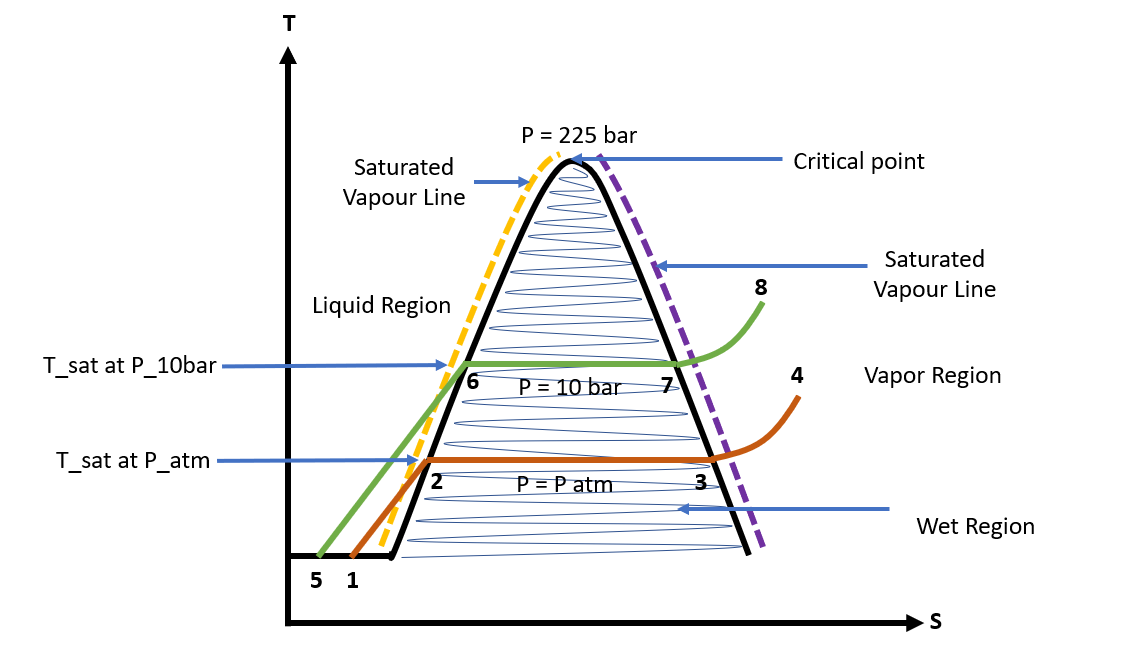
\includegraphics[scale=0.5]{Phasechange.png}
			\centering
		\end{figure}
		\item Terms:
			\begin{itemize}
				\item $s_f$ = Specific entropy of saturated water
				\item $s_g$ = Specific entropy of saturated vapor
				\item $s_{fg} = s_g - s_f$ = Specific entropy change during the phase change $\impliedby$ (becomes zero at Critical point) 
			\end{itemize}
	\end{itemize}\hrulefill\\\\
%----------------------------------------------------------------------------------------%
\dashuline{\textbf{Property Diagrams}}\\\\
\textsc{P-T diagram}
	\begin{itemize}
		\item Also called Phase diagram
		\item Three lines separates the three phases
			\begin{itemize}
				\item \textbf{Sublimation line: }separates Solid and vapour
				\item \textbf{Vapourization line: }separates Liquid and Vapour
				\item \textbf{Melting (or) Fusion line: }separates Solid and Liquid
					\begin{itemize}
						\item Substances that expand or contract on freezing differ only in the Melting line of the PT diagram.
					\end{itemize}
			\end{itemize}
		\item The above three lines meet at \textbf{Triple Point}.\textbf{NOTE: } Only in P-T diagram, there is no phase change region and as a result, the triple point exists as point. In all other diagrams, there is phase change region and the triple point exists as a line and so its called as \textbf{Triple line}
		\item But critical point is a point in all the diagrams, no exceptions. 
		\end{itemize}\hrulefill\\\\
%----------------------------------------------------------------------------------------%
\textsc{h-s diagram (or) Mollier Diagram}
	\begin{itemize}
		\item We know, $Tds = dh - vdP \implies Tds = dh$ (at Constant pressure $dP=0$) $\implies \boxed{\left(\dfrac{dh}{ds}\right)_{P} = T}$
		\item In wet region of h-s diagram, isotherms and isobars are same and they start deviating when they enter the superheated region. 
		\item The slope of an isobar on the h-s coordinate is equal to the absolute temperature at that pressure
		\item Terms:
			\begin{itemize}
				\item $h_f$ = Specific enthalpy of saturated water at a given pressure
				\item $h_g$ = Specific enthalpy of saturated vapor at a given pressure
				\item $h_{fg}$ = Latent heat of vaporization at a given pressure. As the pressure increases, $h_{fg}$ decreases and becomes zero at critical point.
			\end{itemize}
	\end{itemize}\hrulefill\\\\
%----------------------------------------------------------------------------------------%
\dashuline{\textbf{Quality and Saturated Liquid-Vapor Mixture :-}}
	\begin{itemize}
		\item \textbf{Dryness fraction(x) = }$\dfrac{mass\;of\;saturated\;vapor}{total\;mass}\implies\boxed {x = \dfrac{m_g}{m_f+m_g}}\;\;(0\le x\le1)$
		\begin{itemize}
			\item[$\implies$] x=0 for saturated liquid 
			\item[$\implies$] x=1 for saturated vapor
			\item[$\implies$] If x $>$ 1 in any problem, then it's in Superheated region.
			\item[$\implies$] If x $<$ 0 in any problem, then it's in Subcooled region.
			\item x is undefined at critical point. 
			\item Consdier:
				\begin{itemize}
					\item A mixture of saturated liquid and saturated Vapor
					\item Total Mass (m) = $m_f + m_g$
					\item Total Volume (V) = $V_f + V_g \implies m_fv_f + m_gv_g \implies v = \dfrac{V}{m} \implies \dfrac{m_fv_f}{m} + \dfrac{m_gv_g}{m}$
					\item $v = (1-x)v_f + xv_g \impliedby \boxed{\dfrac{m_f}{m} = \dfrac{m-m_g}{m} = 1 - \dfrac{m_g}{m} = 1 - \dfrac{m_g}{m_f+m_g} = 1 - x}$
					\item $v=v_f-xv_f+xv_g \implies v_f + x(v_g-v_f) \implies \boxed{\bm{v =  v_f+xv_{fg}}}$
					\item Now instead of volume, had any other property been taken, they all would end with the similar result as above, meaning: The value of any specific-extensive property(y) in the wet region is $y = y_f+x(y_{fg})$
					\item[$\implies$] $\boxed{h=h_f+x(h_{fg})}\;\boxed{s=s_f+x(s_{sg})}\; \boxed{u=u_f+x(u_{ug})}$
					\item $\boxed{\bm{Lever\;Rule:\;}\;x = \dfrac{y-y_f}{y_{fg}}}$
				\end{itemize}
		\end{itemize}		 
	\end{itemize}\hrulefill\\\\
%----------------------------------------------------------------------------------------%
\dashuline{\textbf{Enthalpy and Entropy of Pure substances :-}}	\\\\
\textsc{Enthalpy at Various Points}
	\begin{itemize}
		\item \underline{Wet region:} $\boxed{h = h_f + x(h_{fg})}$
		\item \underline{Superheated region:} $\boxed{h = h_g + C_{pv}(T-T_{sat})} \impliedby C_{pv} =\;$Specific heat of superheated vapor at Const P
		\item \underline{Subcooled region:} $\boxed{h = h_f+C_{pl}(T_{sat}-T)} \impliedby C_{pl} =\;$Specific heat of subcooled liquid at Const P
	\end{itemize}
%----------------------------------------------------------------------------------------%
\textsc{Entropy at Various Points}
	\begin{itemize}
		\item \underline{Wet region}:
			\begin{itemize}
				\item[$\rightarrow$] $s = s_f+x(s_fg) \impliedby s_{fg} = (s_g - s_f)$ = Entropy of Vapourization
				\item[$\rightarrow$] Evaporation is an Isothermal process and we know $ds = (s_g - s_f)=\dfrac{\delta Q}{T}$
				\item When a liquid evaporates, the heat absorbed is the latent heat of vaporization ($h_{fg}$) and thus heat goes into water without showing any rise in temperature $\implies Q = h_{fg} \implies \boxed{s_{fg} = s_{evap} = \dfrac{h_{fg}}{T_{sat}}}$ 
			\end{itemize}
		\item \underline{Supherheated region:}
			\begin{itemize}
				\item[$\rightarrow$] We know $Tds = dh - vdP \implies Tds = c_{pv}dT \impliedby$ ($dp=0$ at constant pressure and $dh = c_{pv}dT$)
				\item[$\rightarrow$] $ds = \dfrac{c_{pv}dT}{T}$ Integrating, $s_2-s_g = \int\limits_g^2\dfrac{c_{pv}dT}{T} \implies c_{pv}\ln\left(\dfrac{T_2}{T_g}\right)$
				\item[$\rightarrow$] $\implies \boxed{s_2 = s_g + c_{pv}\ln\left(\dfrac{T_2}{T_{sat}}\right)}$ as ($T_f=T_g=T_{sat}$)
			\end{itemize}
		\item \underline{Subcooled region:}
			\begin{itemize}
				\item[$\rightarrow$] Similar to the above derivation. So, $\boxed{s_3 = s_f + c_{pl}\ln\left(\dfrac{T_{sat}}{T_3}\right)}$
			\end{itemize}
	\end{itemize}\hrulefill\\\\
%----------------------------------------------------------------------------------------%
\dashuline{\textbf{Points to remember :-}}
	\begin{itemize}
		\item Always remember to taken in account the mass when dealing with pure substance problems
		\item Energy supplied in constant volume will be the change in Internal energy
		\item Energy supplied in constant pressure will be the change in Enthalpy
		\item The values u,h, and s cannot be measured directly and they are calculated from measurable properties using the relations between thermodynamic properties. But those relations give the changes in properties and not the actual values of the properties at specified state. Therefore a reference state is chosen and that property is assigned a value of zero at that state. 
			\begin{itemize}
				\item[$\rightarrow$] For water, a state of saturated liquid at 0.01\textdegree C is taken as reference
				\item[$\rightarrow$] Some properties may have negative values as a result of the chosen reference state. It should be noted that different tables list different values for some properties at the same state as a result of using different reference state. 
			\end{itemize}
	\end{itemize}\hrulefill\\\\
%----------------------------------------------------------------------------------------%
\begin{center}
\subsection*{\uwave{8. Thermodynamic Relations}}
\end{center}
\dashuline{\textbf{Mathematical Theorems :-}}\\
	\begin{itemize}
		\item $\left(\dfrac{\delta P}{\delta v}\right)_T\left(\dfrac{\delta T}{\delta P}\right)_v\left(\dfrac{\delta v}{\delta T}\right)_P = -1 \impliedby$ by Chain rule
	\end{itemize}\hrulefill\\\\
%----------------------------------------------------------------------------------------%
\dashuline{\textbf{Maxwell Relations :-}}
	\begin{itemize}
		\item The equations that relate the partial derivatives of properties P,v,T and s of a simple compressible system to each other are called Maxwell relations. 
		\item They are obtained from 4 Gibbs equations in which 2 of them we have already seen by the name of TdS equations. 
			\begin{align}
				du &= Tds - Pdv\\
				dh &= Tds + vdP
			\end{align}
		\item The other 2 gibbs functions are derived from:
			\begin{align}
			 	f = u - Ts \tag{a}\\
			 	g = h - Ts \tag{b}
			\end{align}
		\item Here $f$ is calld \textbf{Helmholtz function} and $g$ is called \textbf{Gibbs function} and for any natural process, both these values decrease and attain a minimal value.
		\item By differentiating (a) and (b), we get, $df = du - Tds - sdT$ and $dg = dh - Tds - sdT$. using $du - Tds = -Pdv$ and $dh - Tds = vdP$ from (1) and (2) we get the remaining 2 gibbs relations:
		\begin{align}
			df &= -sdt -Pdv\\
			dg &= -sdT + vdP
		\end{align}
		\item Using the exact differential, $\left(\dfrac{\delta M}{\delta z}\right)_y = \left(\dfrac{\delta N}{\delta y}\right)_z$ on the four relations we'll obtain:
		\item $\boxed{\left(\dfrac{\delta T}{\delta v}\right)_s = -\left(\dfrac{\delta P}{\delta s}\right)_v}\;\;  \boxed{\left(\dfrac{\delta T}{\delta P}\right)_s = \left(\dfrac{\delta v}{\delta s}\right)_P}\;\;  \boxed{\left(\dfrac{\delta s}{\delta v}\right)_T = \left(\dfrac{\delta P}{\delta T}\right)_v}\;\;  \boxed{\left(\dfrac{\delta s}{\delta P}\right)_T = -\left(\dfrac{\delta v}{\delta T}\right)_P}$
		\item The above 4 are the Maxwell relations which are extremely important as they provide a mean to determine the change in entropy which is not possible by simply measuring the properties P, v and T
	\end{itemize}\hrulefill\\\\
%----------------------------------------------------------------------------------------%
\dashuline{\textbf{Tds Partial Differential Equations :-}}
	\begin{itemize}
		\item $\boxed{Tds = C_vdT + T\left(\dfrac{\delta P}{\delta T}\right)_vdV}$
		\item $\boxed{Tds = C_pdT - T\left(\dfrac{\delta V}{\delta T}\right)_PdP}$
		\item The above two are derived by writign s =$f$(T,v) and s=$f$(T,P) and then applying Maxwell relations
	\end{itemize}\hrulefill\\\\
%----------------------------------------------------------------------------------------%
\dashuline{\textbf{Specific Heats $C_p$ and $C_v$}}
	\begin{itemize}
		\item $\boxed{\beta = \dfrac{1}{v}\left(\dfrac{\delta v}{\delta T}\right)_P}\;\;\;$ $\boxed{K_T = \dfrac{-1}{v}\left(\dfrac{\delta v}{\delta P}\right)_T}\;\;\;$ $\boxed{C_p-C_v = \dfrac{Tv\beta^2}{K_T}}$
		\item $K_T$ = Isothermal Compressibility
		\item $\beta$ = Volume expansivity
	\end{itemize}\hrulefill\\\\
%----------------------------------------------------------------------------------------%
\dashuline{\textbf{Energy and Enthalpy Equations :-}}
	\begin{itemize}
		\item $\boxed{du = C_vdT + \left[T\left(\dfrac{\delta P}{\delta T}\right)_v-P\right]dv}\;\;\; \boxed{dh = C_pdT - \left[T\left(\dfrac{\delta v}{\delta T}\right)_P-v\right]dP}$
	\end{itemize}\hrulefill\\\\
%----------------------------------------------------------------------------------------%
\dashuline{\textbf{Joule Thomson Coefficient :-}}
	\begin{itemize}
		\item When a fluid passes through a restriction such as a porous plug, a capillary tube or an ordinary valve, its pressure decreases due to throttling. Although this \textbf{throttling is Isenthalpic}, the temperature behaviour of the fluid during the throttling is described by the Joule-thomson coefficient($\mu$)
		\item$\boxed{\mu = \left(\dfrac{\delta T}{\delta P}\right)_h}$
			\begin{itemize}
				\item[$\rightarrow$] $\mu > 0 \implies$ Temperature increases during throttling
				\item[$\rightarrow$] $\mu < 0 \implies$ Temperature decreases durign throttling
				\item[$\rightarrow$] $\mu = 0 \implies$ Temperature remains constant durign throttling
				\item[$\rightarrow$] There will be no change in temperature when Ideal gas is throttled.
			\end{itemize}
	\end{itemize}\hrulefill\\\\
%----------------------------------------------------------------------------------------%
\dashuline{\textbf{Clausius - Clapeyron Equation :-}}
	\begin{itemize}
		\item Clausius clapeyron gives the relation between the $P_{sat}, T_{sat}$, Enthalpy of evaporation and the specific volume of the two phases involved. 
		\item[$\implies$] $\boxed{\left(\dfrac{\delta P}{\delta T}\right)_{sat} = \dfrac{h_{fg}}{T_{sat}v_g}} = \boxed{\dfrac{h_{fg}P_{sat}}{RT_{sat}^2}}$
	\end{itemize}
%----------------------------------------------------------------------------------------%
\dashuline{\textbf{Compressibility Factor(z) :-}}
	\begin{itemize}
		\item $Z = \dfrac{Actual\;Volume}{Ideal\;Gas\;Volume} = \dfrac{V_a}{V_i} = \dfrac{Pv_a}{RT}$
		\item If a gas behaves like an ideal gas then Z=1 at all temperatures and pressures. 
		\item Z is used to quantify the deviation of gases from ideal gas behaviour.
		\item Reduced Pressure$(P_r = \dfrac{P}{P_C})$ is the ratio of existing pressure to Critical pressure. Similarly, $T_r = \dfrac{T}{T_C}$ and $v_r = \dfrac{v}{v_C} = \dfrac{Z}{Z_C}\dfrac{T_r}{P_r}$
		\item The deviation is highest in the vicinity of critical point. 
		\item At very low pressure or very high temperature Ideal gas behaviour can be assumed.
	\end{itemize}\hrulefill\\\\
%----------------------------------------------------------------------------------------%
\dashuline{\textbf{Van der Waal's Equation of state :-}}
	\begin{itemize}
		\item $\boxed{\left(P_C+\dfrac{a}{V_c^2}\right)(V_c-b) = RT_C}$
			\begin{itemize}
				\item[$\rightarrow$] $v_c = 3b$
				\item[$\rightarrow$] $T_C = \dfrac{8}{27Rb}$
				\item[$\rightarrow$] $P_C = \dfrac{a}{27b^2}$
				\item[$\rightarrow$] $a = \dfrac{27R^2T_C^2}{64P_C}$
				\item[$\rightarrow$] $b = \dfrac{RT_C}{8P_C}$
				\item[$\rightarrow$] At critical point, $\dfrac{P_Cv_c}{RT_C} = \dfrac{3}{8}$
			\end{itemize}
	\end{itemize}\hrulefill\\\\\
%----------------------------------------------------------------------------------------%
\end{document}
